\documentclass{article}

% Please use the following line and do not change the style file.
\usepackage{icml2021_author_response}

% Recommended, but optional, packages for figures and better typesetting:
\usepackage{microtype}
\usepackage{graphicx}
\usepackage{subfigure}
\usepackage{hyperref}       % hyperlinks
\usepackage{booktabs} % for professional tables
\usepackage{amsfonts}       % blackboard math symbols
\usepackage{nicefrac}       % compact symbols for 1/2, etc.

\usepackage{lipsum}

\begin{document}
% Uncomment the following line if you prefer a single-column format
% \onecolumn

First of all we would like to sincerely thank all reviewers for their very detailed and precise remarks on our work. These comments are very useful to improve many aspects of the article, both on theoretical and numerical points.
\begin{figure}[H]
\vskip -0.1in
\begin{center}
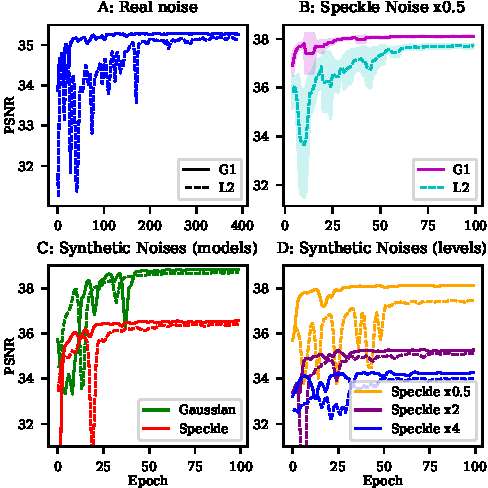
\includegraphics[width=\columnwidth]{fig_review.pdf}
\vskip -0.15in
\caption{PSNR is computed at each epoch on the evaluation dataset during the training of our network including NNet (G1) or DNet only (L2). A: training on real noise. Final performance gain of G1 over L2 is $+0.11dB$. C, D: training on different model/levels of synthetic noise added to ground truth image. C: \textit{Gaussian} and \textit{Speckle} correspond to noises presented in section 5.1, that have no and high signal dependency respectively. D: \textit{Speckle} x0.5, x2, x4 correspond to \textit{Speckle} condition with variance multiplied by 0.5, 2 and 4 respectively. B: Mean and SEM over 5 runs. In order to speed up analysis: trainings in B,C \& D are performed with 100 epochs and decrease on plateau of 10 epochs (instead of 30); PSNR are computed without flip/transposition invariance.}
\label{fig:review}
\end{center}
\vskip -0.25in
\end{figure}
\paragraph{CONTRIBUTION OF NNET}
We agree that in its original version the several contributions presented in the paper are not properly distinguished. In the revised manuscript, we propose to highlight the contribution of the N-net to the performance.
Fig.~\ref{fig:review}~(A, C, D) shows the impact of the noise net on real and several levels of synthetic noise, by comparing our model with the D-Net trained with L2 loss (as in N2V, N2S) with every other aspect fixed. It shows that NNet always improves performances, although not always significantly (this is the case for all datasets considered in the article). Moreover the addition of N-net greatly stabilizes the training (As shown in Fig.~\ref{fig:review}~B) and improves convergence speed, which enables easier hyperparameters and architecture optimization. We also noticed that introducing NNet provides robustness to variations in signal scaling. The noise model alone can thus be seen as a modular and plug-and-play addition to existing blind denoising models, which always improves performances and convergence.

From the perspective of our framework, the L2 loss can be understood as a particular case of the NNet predicting a constant unit gaussian noise. When the actual noise is significantly different from it (speckle vs constant gaussian for instance), our N-net has a stronger impact, as shown in the middle plot.
TODO SYLVAIN  Intuitively, better knowledge of the noise gives better prediction of X (it is known that misspecifying the noise density can lead to very poor mean integrated squared error (MISE) of the deconvolution estimator of the signal distribution, see XXX).

Moreover the noise model was shown in the main paper to capture several statistical behaviors, which is interesting \textit{per-se} and could allow to further improve performances by predicting signal distribution as in works like Laine et al. 2019 and PN2V.

\paragraph{THEORY}
R2 concerns about the way the loss function is described in the original version of the paper indicate that we did not provide enough details to support the proposed loss. This loss function is obtained as an approximation of the negative loglikelihood of the model which will be stated clearly in the revised version as follows.
%The D-net $\mu_\theta(\Omega_y,g(\Omega_y))$ is indeed thought as a model for the expected value of the signal X given the surrounding receptive field excluding the central pixel. This quantity as an estimate of the signal value would indeed minimize the mean squared error to the ground truth and this is what supervised training with MSE does.
The conditional loglikelihood of the observations is written $ \log p(y|\Omega_y) = \log \int p(x,y|\Omega_y) \mathrm{d}x = \log \int p(x|\Omega_y)p(y|\Omega_y,x) \mathrm{d}x$ (***), where $p(y|\Omega_y,x)$ is given by our observation model (1).
As it is very challenging to obtain samples from the distribution $p(x|\Omega_y)$ we propose indeed to estimate this integral by $\log p(y|\Omega_y,\hat {x})$ where $\hat {x}$ is an estimate of $\mathbb{E}[X|\Omega_y]$. Our loss function is then supported by the intuition that $\mu_\theta(\Omega_y,g(\Omega_y))$ is a good approximation of $\mathbb{E}[X|\Omega_y]$. Providing theoretical guarantees  that this approximation is good remains an open problem as stated in the original paper. Even though this seems similar to N2V and N2S in terms of loss function we would like to stress that writing explicitly (***) provides a different perspective which we believe:
(1) defines a framework to justify theoretically the proposed approximation (which in our opinion is a challenging issue); (2) highlight in (***) the contribution of $\mu_\theta$ and of the noise model.

\paragraph{SUPERVISED LEARNING}
Following the recommendation of R1 and R2, we compared our method to the supervised approach on dataset W2S-1,2 \& 3 where the evaluation dataset is distinct from the training dataset. We found that our method outperforms the supervised approach of $0.11dB$, $0.22dB$ and $0.26dB$ respectively. This is not in contradiction with the fact that the central pixel is masked at train time. Indeed, as our method actually uses beneficially the central pixel at inference.

\paragraph{NOISE CORRELATION}
Regarding the question of R4: only 2 of the 6 dataset display correlation in noise, that is emphasized by the network when not taken into account. Following (Broaddus et al. 2020) we adapted our masking scheme to take this correlation into account (see section 4.3).

\paragraph{LITERATURE}
We thank R2 for pointing out erroneous analysis of Krull et al., 2019, and will update the manuscript accordingly.
Regarding Prakash et al., 2020a, it seems that joint learning of noise model was introduced in the pre-print version of March 1st, so after we submitted the manuscript. We will take into account this change and update the manuscript accordingly.
% [To be removed si besoin de place] Additionally they model the noise variance as an affine function of the signal intensity. We show that the noise variance may follow a more intricate dependency to the signal intensity and design a more general way to model it
\end{document}
